\documentclass{article}
\usepackage{graphicx,amssymb,amsmath,amsthm,biblatex,subfig,float,multirow} % Required for inserting images
\addbibresource{[BIBLIOGRAPHY].bib}
\title{ME489 Homework 1}
\author{Mustafa Yiğit Görgün \\ 2446094}
\date{October 27th 2023}

\begin{document}

\maketitle
\begin{abstract}
For the numerical simulation of multiscale problems, Higher Order (HO) systems and one their discretization variants, discontinuos Galerkin Schemes are utilized due their many advantages in the field. In order to utilize these advantages it is necessary to create pre and post processing algorithms that are particularly created with HO in mind. To this day HO support in commercial closed-sourced software are far from enough. In this paper researchers showcase the FLEXI framework which is HO consistent and open-sourced simulation tool chain. By fusing the DG-based solver for the Navier-Stokes equations, a mesh generator tool (HOPR) and the post-processing suite (POSTI) FLEXI offers a toolset for fluid dynamics simulations. In this article the FLEXI, its core numerical algorithms, features and capabilities of its framework are discussed. 
\end{abstract}
\section{Summary}
The FLEXI framework consists of open-source tools for pre-processing and generation of high order meshes,
the CFD solver itself and a post-processing and visualization suite. The tool used for mesh input file generation is HOPR. This tool is used for surface and volume curving of the meshes. For surface curving two different approaches can be taken with this tool: surface-subdivision and point-normal. The surface-subdivision approach is the easiest approach but it requires additional programs and meshes to work properly. The difference between using and not using this approach can be seen in Fig. 1. 
\begin{figure}[H]
\begin{center}
\subfloat{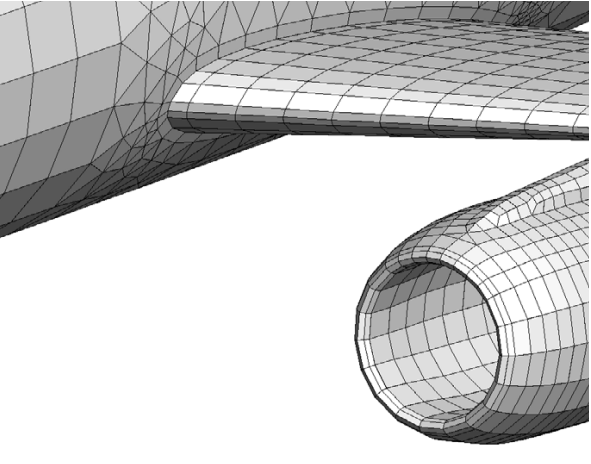
\includegraphics[width=0.5\textwidth]{figures/Screenshot from 2023-10-27 03-30-40.png}}\hfill
\subfloat{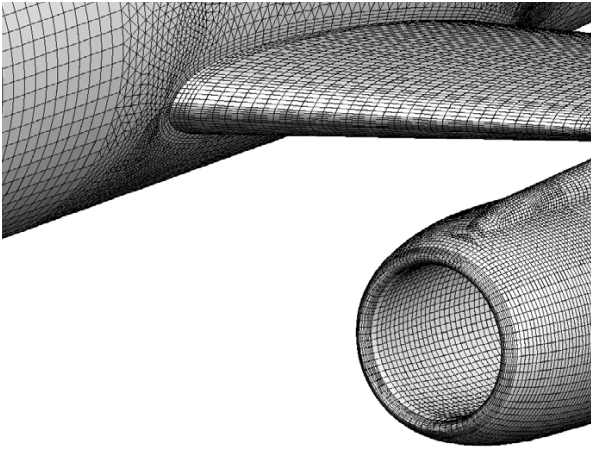
\includegraphics[width=0.5\textwidth]{figures/Screenshot from 2023-10-27 03-30-53.png}}
    \caption{Surface mesh of an example surface before and after using surface-subdivision strategy.}
    \label{Figure1.fig}
\end{center}
    

\end{figure}
The point-normal approach needs to reconstruct the surface by the provided normal vectors. The methodology of this approach can be seen in Fig.2. 
\begin{figure}[H]
    \centering
    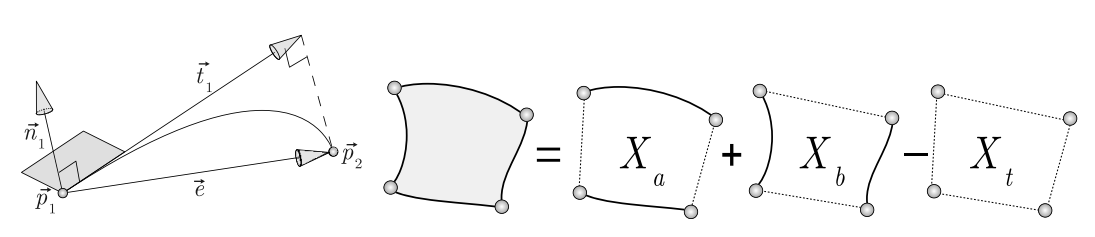
\includegraphics[width=1\linewidth]{figures/image_2023-10-27_035316780.png}
    \caption{Construction of curved edge tangential from point-normal vector (left) and blending of curved edges to curved surface (right)}
    \label{Figure2.fig}
\end{figure}
As for the numerical methods used primarily Discontinous Galerkin Spectral Element Method is mentioned by Krais et al \cite{hellur}. The derivation of this method in the paper starts with a form of conservation law in terms of the convective and viscous fluxes $\vec{F}^c$ and $\vec{F}^v$ respectively and conserved variables $\vec{U}$ defined on some domain $\Omega \subseteq \mathbb{R}$:
\begin{equation}
     \frac{\partial \vec{U}(\vec{x}, t)}{\partial t}+\nabla \cdot\left(\vec{F}^c(\vec{U})-\vec{F}^v(\vec{U}, \nabla \vec{U})\right)=0.
\end{equation}
The derivation of this method ends with the result of:
\begin{align}
\overrightarrow{\mathrm{g}}{i j k}^d=\frac{1}{\mathcal{J}{i j k}} & {\left[\sum_{\alpha=0}^N \overrightarrow{\mathrm{u}}{\alpha j k}^{1, d} \hat{D}{i \alpha}+\left(\left[\vec{U}^* \hat{n}d \hat{s}\right]{j, k}^{+\xi^1} \hat{\ell}i(1)+\left[\vec{U}^* \hat{n}_d \hat{S}\right]{j, k}^{-\xi^1} \hat{\ell}_i(-1)\right)\right.} \\
& +\sum_{\beta=0}^N \vec{u}{i \beta k}^{2, d} \hat{D}{j \beta}+\left(\left[\vec{U}^* \hat{n}d \hat{s}\right]{i, k}^{+\xi^2} \hat{\ell}j(1)+\left[\vec{U}^* \hat{n}_d \hat{S}{i, k}^{-\xi^2} \hat{\ell}_j(-1)\right)\right. \\
& \left.+\sum_{\gamma=0}^N \vec{u}{i j \gamma}^{3, d} \hat{D}{k \gamma}+\left(\left[\vec{U}^* \hat{n}d \hat{S}\right]{i, j}^{+\xi^3} \hat{\ell}k(1)+\left[\vec{U}^* \hat{n}_d \hat{S}\right]{i j}^{-\xi^3} \hat{\ell}_k(-1)\right)\right] \forall i, j, k .
\end{align}
Where,
\begin{equation}
    \vec{U}^*=\frac{1}{2}\left(\vec{U}_L+\vec{U}_R\right).
\end{equation}
and
\begin{equation}
    \vec{F}^{v *}=\frac{1}{2}\left(\vec{F}^v\left(\vec{U}_L, \vec{g}_L\right)+\vec{F}^v\left(\vec{U}_R, \vec{g}_R\right)\right).
\end{equation}
\begin{table}[H]
\begin{center}
    
\caption{Maximum and minimum velocities along the center lines with different weight ratios of
residual loss and the boundary loss.}
\label{table:1}
\begin{tabular}{ccccccc}
\hline 
\hline 
\multirow{2}{*}{$\omega_R / \omega_{B C}$} 
& \multicolumn{2}{c}{$R a=10^3$} 
& \multicolumn{2}{c}{$R a=10^4$} 
& \multicolumn{2}{c}{$R a=10^5$} \\
\cline { 2 - 7 } 
& $u_{\max }$ 
& $v_{\max }$ 
& $u_{\max }$ 
& $v_{\max }$ 
& $u_{\max }$ 
& $v_{\max }$ \\
\hline 
\hline 0.5 & 0.137 & 0.138 & 0.190 & 0.231 & 0.137 & 0.273 \\
1 & & & 0.192 & 0.233 & 0.128 & 0.258 \\
2 & & & & & 0.132 & 0.261 \\
4 & & & & & 0.130 & 0.261 \\
\hline 
\hline
\end{tabular}
\end{center}
\end{table}
\printbibliography
\end{document}
